% Build from this directory:
% latex -interaction=nonstopmode -halt-on-error pam-5.tex
% dvisvgm --no-fonts --exact --bbox=papersize pam-5.dvi -o pam-5.svg
\documentclass[tikz,border=4pt]{standalone}
\usetikzlibrary{arrows.meta}
\begin{document}
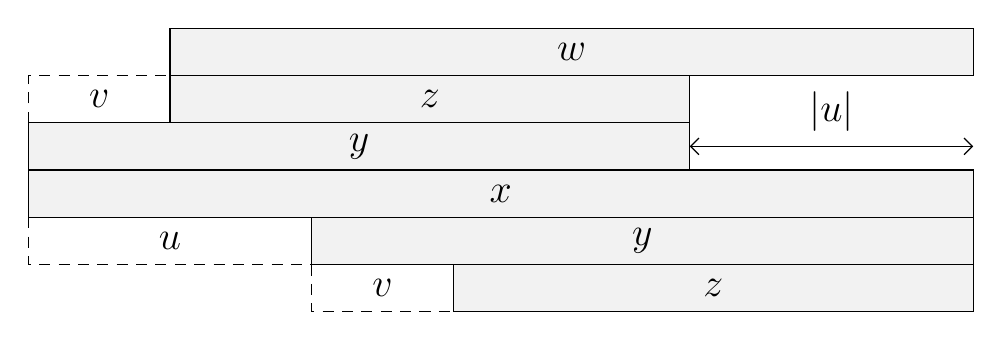
\begin{tikzpicture}[line width=0.45pt,font=\fontsize{14}{17}\selectfont,
  part/.style={fill=black!5},omitted/.style={dash pattern=on 4pt off 3pt}]
  % The top and bottom decompositions share the same interval x.
  % x = vw = uy and y = vz; the two copies of z are a border of w.
  \draw[part] (1.8,1.8) rectangle (12,1.2);
  \draw[part] (1.8,1.2) rectangle (8.4,0.6);
  \draw[part] (0,0.6) rectangle (8.4,0);
  \draw[part] (0,0) rectangle (12,-0.6);
  \draw[part] (3.6,-0.6) rectangle (12,-1.2);
  \draw[part] (5.4,-1.2) rectangle (12,-1.8);
  \draw[omitted] (0,0.6) -- (0,1.2) -- (1.8,1.2);
  \draw[omitted] (0,-0.6) -- (0,-1.2) -- (3.6,-1.2);
  \draw[omitted] (3.6,-1.2) -- (3.6,-1.8) -- (5.4,-1.8);
  \draw[{Straight Barb[length=3pt]}-{Straight Barb[length=3pt]}]
    (8.4,0.3) -- node[above=2pt] {$|u|$} (12,0.3);
  \node at (6.9,1.5) {$w$};
  \node at (0.9,0.9) {$v$};
  \node at (5.1,0.9) {$z$};
  \node at (4.2,0.3) {$y$};
  \node at (6,-0.3) {$x$};
  \node at (1.8,-0.9) {$u$};
  \node at (7.8,-0.9) {$y$};
  \node at (4.5,-1.5) {$v$};
  \node at (8.7,-1.5) {$z$};
\end{tikzpicture}
\end{document}
